
\chapter{Instrumentation and data description}
\label{chap:data}
%COFI -- chapter outline and flow integration
For analyzing the solar wind and related areas on the Sun, there exist remote instruments, such as solar imagers and coronagraphs, and in-situ instruments, such as magnetometers and plasma spectrometers. The basic principles of the latter are described in this chapter, because the analyses performed in this thesis are based entirely on in-situ measurements -- except of course the sunspot time series.

Different kind of measurements, collected from observatories at a number of locations, are used for the investigations performed in this thesis. In the following sections, I describe these data sets as well: the geomagnetic disturbance index \Kp{}, the solar activity indicator sunspot number (SSN), and the solar wind in-situ data sets. The solar wind in-situ data sets are the near-Earth OMNI data collections, consisting of minutely and hourly data, that is, low resolution OMNI (LRO) and high resolution OMNI (HRO), and the data obtained from the Helios~1 and Helios~2 spacecraft in the 1970s. I prepared a time coverage overview of all data sets in relation to the solar activity cycles in \autoref{fig:timeline_SSN_with_data_and_sc}.
\begin{figure}[htb]
	\centering
	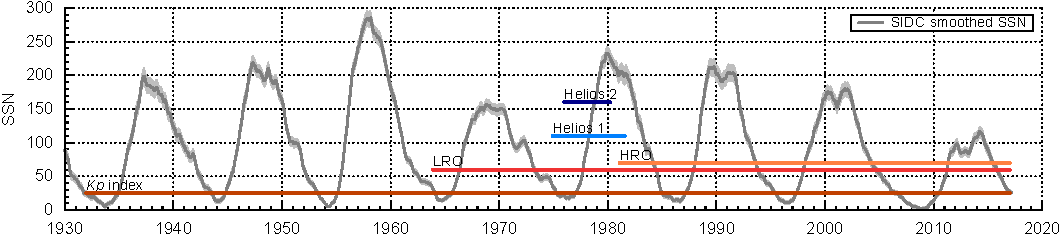
\includegraphics[width=\textwidth]{figures_of_mine/gnuplots/timeline_SSN_with_data_and_sc.pdf}
	\caption[\lofimage{figures_of_mine/gnuplots/timeline_SSN_with_data_and_sc.pdf}I created the figure myself.]
	{Time coverage of the data sets used in this work together with a plot of the solar activity from 1930 until end of 2016. The individual data sets are the \Kp~index, the low and high resolution OMNI (LRO and HRO) collections, and the Helios~1 and Helios~2 data sets. I added the SIDC 13-month smoothed monthly SSN and the solar cycle number in the background for orientation.}
	\label{fig:timeline_SSN_with_data_and_sc}
\end{figure}


\section{Magnetometer}
\label{sec:magnetometer}
A magnetometer monitors the local magnetic field environment. Almost every interplanetary spacecraft carries magnetometers as apart from providing useful information, they also have low weight, low power requirements, and a low data rate compared to other scientific instruments \citep{Ness1970}. There are different magnetometer types -- prevalent types are fluxgate magnetometers for measuring the magnetic field direction and its strength and search coil magnetometers for observing the magnetic flux and detecting waves. Some spacecraft carry both magnetometer types, as is the case with the Helios, Wind, and THEMIS spacecraft. All magnetic field data employed in the present study was measured by fluxgate magnetometers.

% fluxgate magnetometer
A fluxgate magnetometer consists of two coils around a core -- one coil with alternating current. This current is then compared with the current signal induced into the other coil. Without an external magnetic field both current patterns match. However, the core is easier magnetized in direction of an existing external magnetic field, in this case a differing pattern is detected \citep{Ness1970}. Modern fluxgate magnetometers are designed in a ring core geometry with advanced magnetic core materials, such as molybdenum-permalloy.
% http://sprg.ssl.berkeley.edu/impact/instruments_mag.html
Fluxgate magnetometers are directional, therefore they are usually placed in a set of triaxial configuration. In order to minimize the influence of the spacecraft's own magnetic field, the magnetometers are usually placed away from the spacecraft's body, attached on the ends of solar panels or booms -- often actually two redundant sets at opposite sides of the spacecraft.
% ACE/MAG
In case of the Advanced Composition Explorer (ACE) spacecraft, two triaxial fluxgate magnetometers are mounted \SI{4.2}{\meter} from its center \citep{Smith1998}. The MAG instrument, before integration onto the ACE spacecraft, is pictured in \autoref{fig:ACE_fluxgate_magnetometer}. It has a resolution of a few measurements per second and an accuracy of about \SI{0.1}{\nano\tesla}.
\begin{figure}[htb]
	\fcapside[\FBwidth]{
		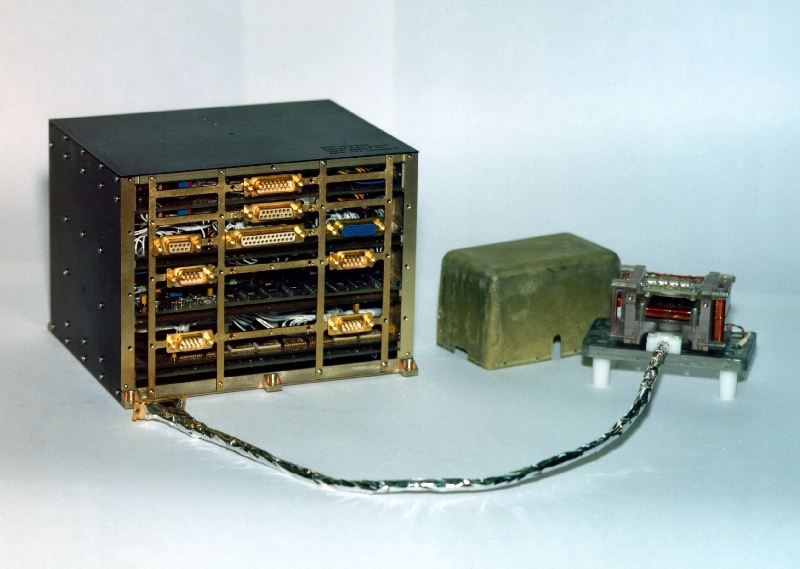
\includegraphics[width=0.6\textwidth]{figures_of_others/images/ACE_fluxgate_magnetometer.jpg}
	}{
		\caption[\lofimage{figures_of_others/images/ACE_fluxgate_magnetometer.jpg}Credit: \href{https://helios.gsfc.nasa.gov/ace/mag.html}{NASA/GSFC}.]
		{MAG instrument from the ACE spacecraft. Pictured is the electronics box and one of the two fluxgate magnetometer sensors. Credit: \href{https://helios.gsfc.nasa.gov/ace/mag.html}{NASA/GSFC}.}
		\label{fig:ACE_fluxgate_magnetometer}
	}
\end{figure}

% Ground based magnetometers measure the local magnetic field of the Earth. They have to be housed in controlled temperature environment and away from magnetic interferences.\\

% % search coil magnetometer
% In a search coil magnetometer one coil is placed around a core; measures plasma waves -- where?\\
% measures magnetic field fluctuations and waves...\\
% measures low frequency magnetic field fluctuations and waves in three directions (tri-axial)\\
% 
% % http://themis.ssl.berkeley.edu/scm_faqs.shtml
% % https://en.wikipedia.org/wiki/Spacecraft_magnetometer
% 
% % https://www.nasa.gov/mission_pages/themis/spacecraft/SCM.html
% ``Search coil magnetometers are basically copper coils wound around a high magnetic permeability core. This magnetic core concentrates magnetic field lines - and the magnetic fluctuations they carry - inside the coils. The fluctuations induce currents and electric voltage drops inside the core that can be measured and recorded by the instrument's electronics circuits.''\\
% 
% search coil magnetometer, see \autoref{fig:searchcoil_magnetometer}\\
% \begin{figure}[htb]
% 	\fcapside[\FBwidth]{
% 		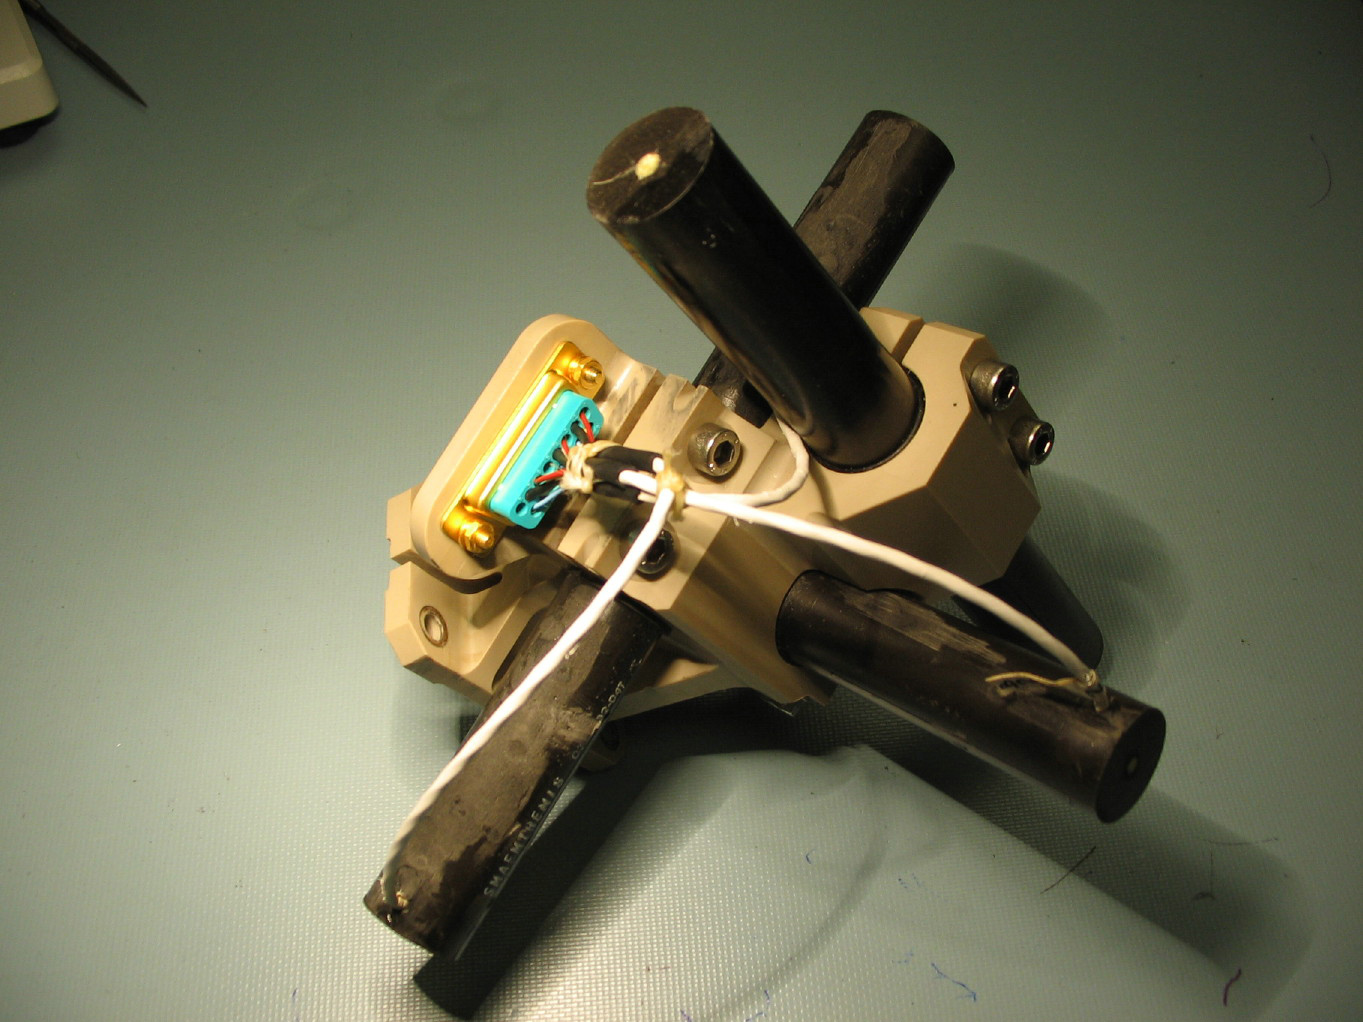
\includegraphics[width=0.5\textwidth]{figures_of_others/images/searchcoil_magnetometer.jpg}
% 	}{
% 		\caption[\lofimage{figures_of_others/images/searchcoil_magnetometer.jpg}]
% 		{Engineering test unit of the search coil magnetometers on the THEMIS satellites launched in 2007. Credit: \href{https://www.nasa.gov/mission_pages/themis/spacecraft/SCM.html}{NASA}, 2007.}
% 		\label{fig:searchcoil_magnetometer}
% 	}
% \end{figure}
% % https://www.nasa.gov/mission_pages/themis/spacecraft/SCM.html
% % https://www.nasa.gov/sites/default/files/thumbnails/image/168038main_scm_etu_1_lg.jpg


\section{Plasma spectrometer}
\label{sec:plasma_spectrometer}
A plasma spectrometer monitors the energy spectrum from a flow of charged particles. These plasma detectors detect the energy spectra and directions of the bulk particle flows. The energy spectra are used to further determine the bulk velocity, temperature, and density. Spectrometers measuring solar wind plasma are specified into electron and ion instruments. There exist several ion spectrometer types which cover different energy ranges for measuring the different solar wind particle species, such as SEPs, and cosmic rays. There are different instrument types for analyzing the masses, elemental composition, isotopic abundances, and charge states.

Solar wind consists almost entirely of protons and alpha ions. The dedicated instruments are built with particle sensors based on Faraday cups or electrostatic analyzers. Faraday cup instruments monitor the solar wind currently on the Wind and DSCOVR spacecraft located near L1, whereas an electrostatic analyzer instrument was in operation on the Ulysses spacecraft. The ACE spacecraft carries the enhanced flight spare instrument from the Ulysses mission.

Electrostatic analyzers are equipped with channel electron multipiers which allow for the detection of every incident particle. However, they only obtain the energy per charge~q. Their energy range is chosen to enclose the proton and alpha ion distributions; in case of the ion spectrometer Solar Wind Electron Proton Alpha Monitor (SWEPAM-I) on board the ACE spacecraft, the energy range is \SIrange{260}{36000}{\electronvolt\per q} \citep{McComas1998a}. An image of the SWEPAM-I instrument is shown in \autoref{fig:ACE_SWEPAM_I}.
\begin{figure}[!b]
	\begin{floatrow}
		\ffigbox{
			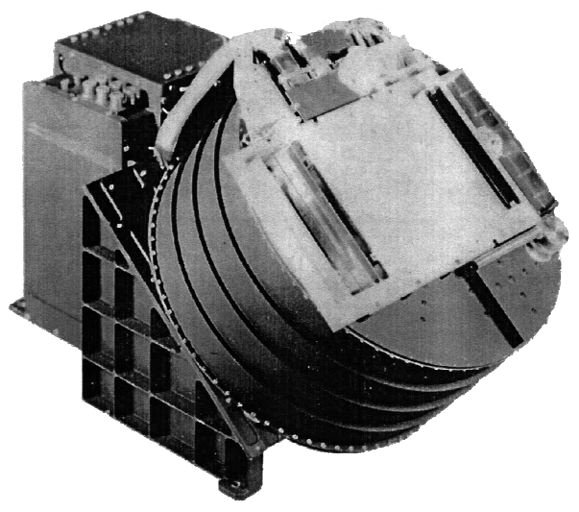
\includegraphics[width=0.4\textwidth]{figures_of_others/images/ACE_SWEPAM_I.jpg}
		}{
			\caption[\lofimage{figures_of_others/images/ACE_SWEPAM_I.jpg}Credit: \href{https://swepam.lanl.gov/}{Los Alamos National Laboratory}.]
			{Ion spectrometer SWEPAM-I onboard the ACE spacecraft. The cylindrical part is the sensor head and the box behind houses the electronics and power supplies. Credit: \href{https://swepam.lanl.gov/}{Los Alamos National Laboratory}.}
			\label{fig:ACE_SWEPAM_I}
			% copyright
			% https://lanl.gov/resources/web-policies/copyright-legal.php
		}
		\ffigbox{
			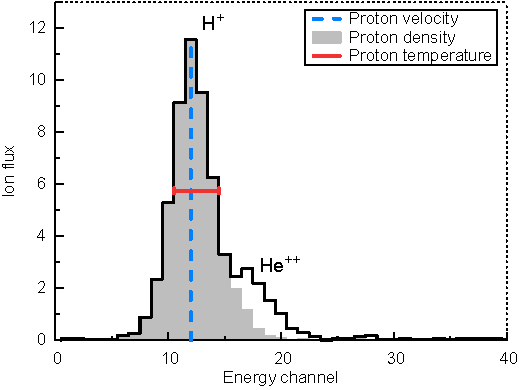
\includegraphics[width=0.46\textwidth]{figures_of_mine/gnuplots/ion_energy_spectrum_b2.pdf}
		}{
			\caption[\lofimage{figures_of_mine/gnuplots/ion_energy_spectrum_b2.pdf}I created the figure myself.]
			{Example of an ion energy spectrum for which I prepared a number of synthetic data points in a way that the helium distribution overlaps with that of the protons. I also indicated the measures of the proton velocity, density, and temperature.}
			\label{fig:ion_energy_spectrum_b2}
			% http://www.goembel.biz/sun.html
		}
	\end{floatrow}
\end{figure}

A plasma ion detector only provides an energy spectrum -- the velocity, density, and temperature of the proton and alpha ions have to be derived from it. Both ion populations can overlap under extremely hot conditions \citep{Bame1992}. The frequency distribution's peak energy indicates the bulk velocity, its area shows the number density, and its width scales with the temperature. I prepared a synthetic ion energy spectrum for illustration in \autoref{fig:ion_energy_spectrum_b2}. The SWEPAM-I experiment calculates these solar wind properties by numerical integration over specified energy ranges. The automatism has its limits (e.g., very low temperatures cannot be assessed correctly), however a manual fit of two superimposed Maxwell-Boltzmann curves to the energy distributions can overcome this \citep{Bame1992}.
% source: ftp://spdf.gsfc.nasa.gov/pub/data/ulysses/plasma/swoops/ion/swoops_ion_users_guide_update_20030214.txt
% ``Plasma parameters are calculated by numerical integration of velocity-weighted
% ion distributions over a E/q range chosen to include the thermal proton and
% alpha-particle populations. Under extremely hot conditions, there can
% sometimes be some overlap between these populations. Additionally, during
% periods when the solar wind temperature is exceptionally low the experiment can
% not properly measure the temperature. Care has been taken to estimate the
% instrument background from channels that do not contain data, and the effects
% of background have been removed from the integration. The velocity space 
% resolution of the experiment is better in the energy dimension than in the
% angular dimensions.''


\section{OMNI data collection}
\label{sec:omni_data_collection}
Solar wind was measured in~situ for the first time by spacecraft in 1959 and since 1963 near-Earth measurements were done almost continuously. The OMNI~2 data collection \citep{King2005} merges data from solar wind magnetic field and plasma, energetic proton fluxes, geomagnetic indices, and solar indices. The included solar wind data starts in 27~November 1963, the temperature data not before 26~July 1965, and is continuously maintained until today. As the data covers decades from multiple spacecraft at varying locations, the solar wind data is composed of intercalibrated data, which has been time-shifted to the nose of the magnetosphere's bow shock upstream of Earth. I created an overview of the various spacecraft contributing to the IMF and solar wind plasma data and their time coverages to the data set in \autoref{fig:timeline_OMNI_SC_IDs}. Especially from the early space age until the 1980s, many different spacecraft contributed to the LRO data set, whereas over the last twenty years, it were only two spacecraft.
\begin{figure}[htb]
	\centering
	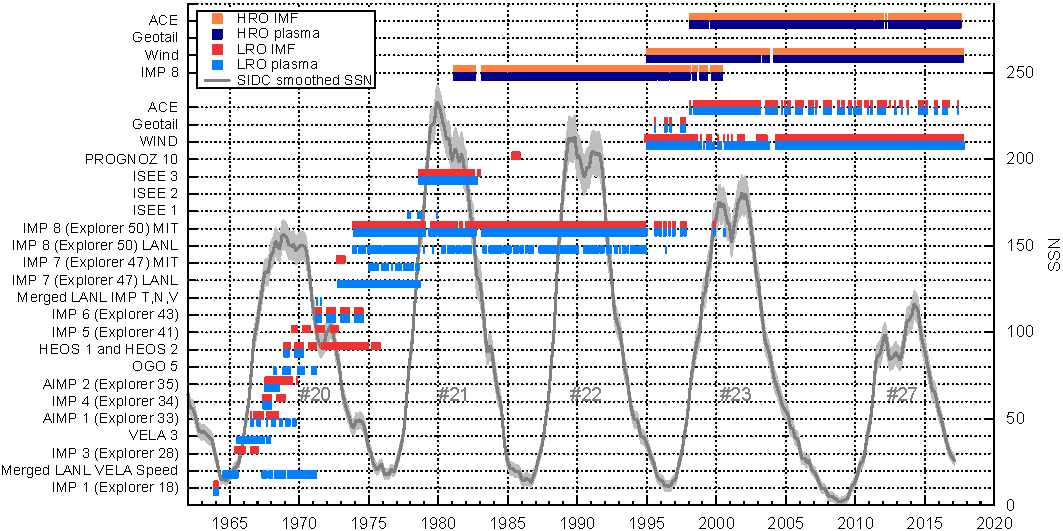
\includegraphics[width=\textwidth]{figures_of_mine/gnuplots/timeline_OMNI_SC_IDs.pdf}
	\caption[\lofimage{figures_of_mine/gnuplots/timeline_OMNI_SC_IDs.pdf}I created the figure myself.]
	{IMF and solar wind plasma data sources (spacecraft) for the high and the low resolution OMNI (HRO and LRO) data sets until the end of 2016. I plotted this figure using the spacecraft identifiers noted in the OMNIWeb Data Documentation\protect\footnotemark. The SIDC 13-month smoothed monthly SSN and the cycle number are plotted in the background.}
	\label{fig:timeline_OMNI_SC_IDs}
\end{figure}
\footnotetext{OMNIWeb Data Documentation: \urlfoot{https://omniweb.gsfc.nasa.gov/html/ow_data.html}}

The OMNI data set is being maintained at NASA's Space Physics Data Facility (SPDF), Goddard Space Flight Center (GSFC). Their OMNIWeb interface \urltext{http://omniweb.gsfc.nasa.gov/} and their Coordinated Data Analysis Web (CDAWeb) interface \urltext{http://cdaweb.gsfc.nasa.gov/} provide the data -- the latter is where I obtained both data sets. The HRO data is used in \autoref{chap:chapter2} for the correlation with the \Kp~index and the LRO data together with Helios data in \autoref{chap:chapterPSP} for the derivation of the solar wind model.

\pagebreak

\section{Helios probes}
\label{sec:helios_probes}
In order to observe solar wind in~situ within the inner heliosphere, the nearly identical solar probes Helios~1 and Helios~2, were launched in December 1974 and January 1976 respectively, one of them is pictured in \autoref{fig:helios2}. Until today, these both probes were the only spacecraft that measured solar wind in~situ over large solar distance ranges with perihelia as close as \SI{0.31}{\au} and \SI{0.29}{\au} respectively. Their highly elliptical orbits in the ecliptic covered a solar distance up to \SI{0.98}{\au}. Launched during solar cycle minimum, the data of both probes cover the rise to the maximum of solar cycle~21, that amounts to about 6.5~years of data at varying solar distances.
\begin{figure}[htb]
	\begin{floatrow}
		\ffigbox[\FBwidth][]{
			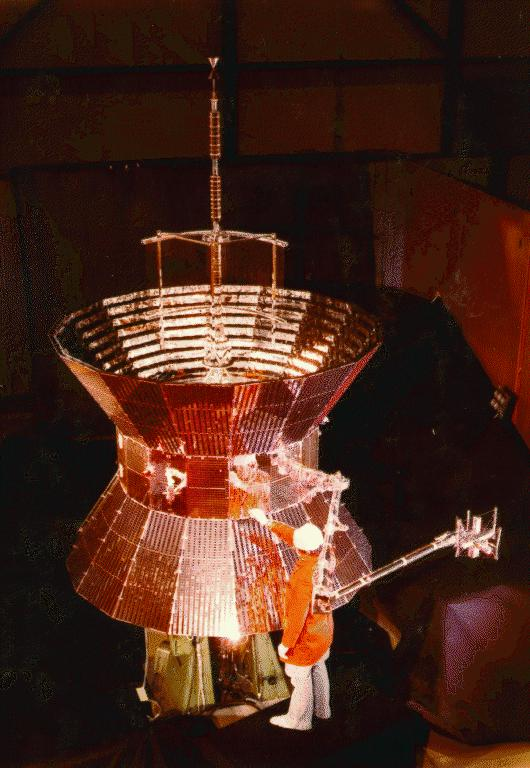
\includegraphics[width=0.3\textwidth]{figures_of_others/images/helios2.jpg}
		}{
			\caption[\lofimage{figures_of_others/images/helios2.jpg}Credit: \href{https://solarsystem.nasa.gov/missions/helios-1/in-depth/}{NASA/Max Planck Institute for Solar System Research}.]
			{One of the nearly identical twin Helios spacecraft\protect\footnotemark. Credit: \href{https://solarsystem.nasa.gov/missions/helios-1/in-depth/}{NASA/Max Planck Institute for Solar System Research}.}
			\label{fig:helios2}
			%source: https://solarsystem.nasa.gov/galleries/helios
			%alternative source: https://solarsystem.nasa.gov/missions/helios-1/in-depth/
			%NASA has no copyrights to its contents (NASA FOIA)
		}
		\ffigbox[\Xhsize]{
			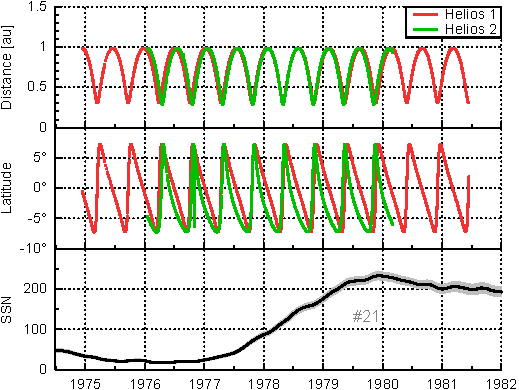
\includegraphics{figures_of_mine/gnuplots/Helios_r_b_ssn.pdf}
		}{
			\caption[\lofimage{figures_of_mine/gnuplots/Helios_r_b_ssn.pdf}I created the figure myself.]
			{Solar distance (top panel) and heliographic latitude (middle panel) of Helios~1 (red) and Helios~2 (green) with respect to their mission time. The trajectory data are from GSFC/SPDF and are plotted in HGI~coordinates. I give the SIDC 13-month smoothed monthly SSN and its cycle number in the bottom panel for orientation.}
			\label{fig:Helios_r_b_ssn}
		}
	\end{floatrow}
\end{figure}
\footnotetext{I was not able to find out which Helios spacecraft this is.}
I plotted the probes' solar distance and heliographic latitude with respect to their mission time and sunspot number for illustration in \autoref{fig:Helios_r_b_ssn}. The daily trajectory data are available from NASA's SPDF at the GSFC\protect\footnote{SPDF Helios~1 trajectory data: \urlfoot{http://spdf.sci.gsfc.nasa.gov/pub/data/helios/helios1/traj/}} and are drawn in Heliographic Inertial (HGI) coordinates, more on HGI coordinates in Appendix~\ref{sec:coordinate_systems}. I also plotted the orbits of Helios~1 and Helios~2 in a solar equatorial plane view and in a solar polar plane view, see \autoref{fig:Helios12_orbits_ecliptic_polar}.
\begin{figure}[t]
	\centering
	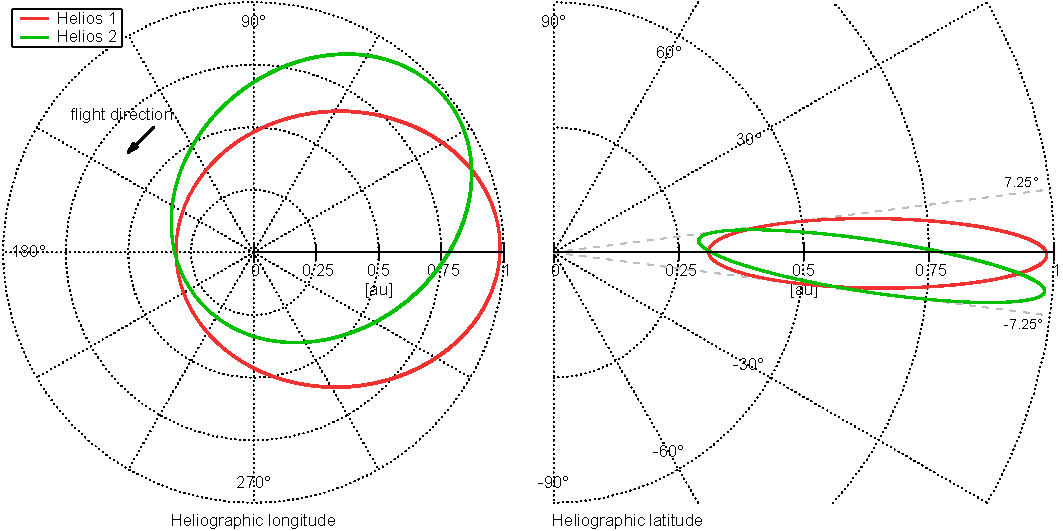
\includegraphics[width=\textwidth]{figures_of_mine/gnuplots/Helios12_orbits_ecliptic_polar.pdf}
	\caption[\lofimage{figures_of_mine/gnuplots/Helios12_orbits_ecliptic_polar.pdf}I created the figure myself.]
	{Orbits of the Helios~1 (red) and Helios~2 (green) spacecraft in the solar equatorial plane (left panel) and in the solar polar plane (right panel). I obtained the trajectory data from GSFC/SPDF and plotted the orbits in HGI~coordinates.}
	\label{fig:Helios12_orbits_ecliptic_polar}
\end{figure}

The scientific instruments carried by the spacecraft for measuring the magnetic field and solar wind plasma are two different fluxgate magnetometers and the Plasma Experiment Investigation. The data from the magnetometer and plasma instruments are merged into a data set with hourly resolution \citep{Rosenbauer1977}. The Helios data is available via the GSFC/SPDF CDAWeb interface: \urltext{http://cdaweb.gsfc.nasa.gov/}. In case of Helios~1 this data set includes about 12.5~orbits in the time range \mbox{1974-12-10} to \mbox{1981-06-14} and in case of Helios~2 about 8~orbits in the time range \mbox{1976-01-01} to \mbox{1980-03-04}. The Helios~1 (Helios~2) magnetometer data coverage, excluding the data gaps, is about \SI{43}{\%} (\SI{54}{\%}) and amounts to 2.8~years (2.3~years) in total, whereas the plasma data coverage is \SI{76}{\%} (\SI{92}{\%}) and amounts to 5.0~years (3.9~years) in total.
The Helios data is used in \autoref{chap:chapterPSP} for analyzing the solar wind parameters' solar distance dependency.

% \begin{figure}[htb]
% 	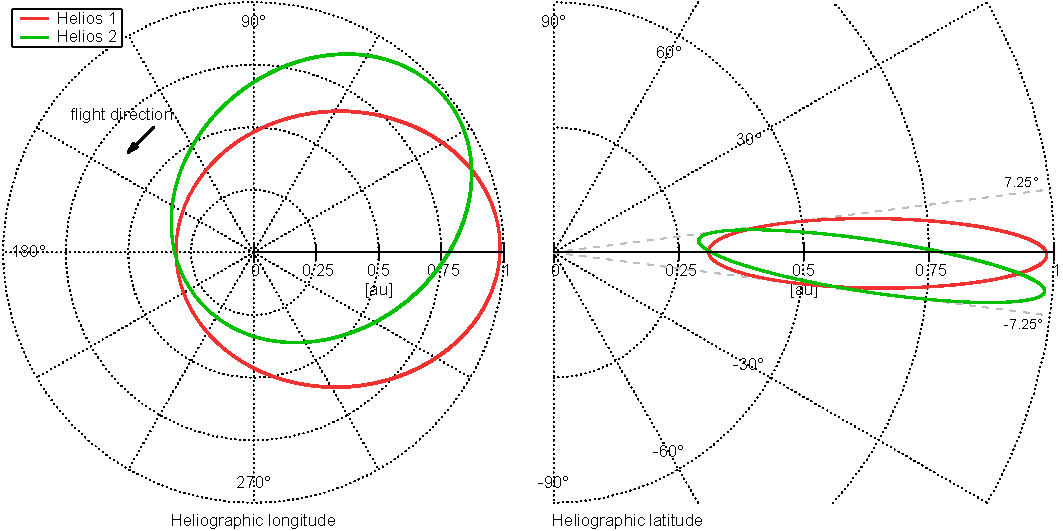
\includegraphics[width=\textwidth]{figures_of_mine/gnuplots/Helios12_orbits_ecliptic_polar.pdf}
% 	\caption[\lofimage{figures_of_mine/gnuplots/Helios12_orbits_ecliptic_polar.pdf}Remove later...]{}
% \end{figure}

%see presi 1.07 Inside Helios-Origins and Evolution-Salem.ppt
%see book Schwenn1990 https://books.google.de/books?id=W1DuCAAAQBAJ&printsec=frontcover&dq=Physics+of+the+Inner+Heliosphere+I.+Large-Scale+Phenomena&hl=de&sa=X&redir_esc=y#v=onepage&q=Physics%20of%20the%20Inner%20Heliosphere%20I.%20Large-Scale%20Phenomena&f=false

% HELIOS~1 and 2 -- orbital Parameters:\\
% \url{http://spdf.sci.gsfc.nasa.gov/pub/data/helios/helios1/traj/}\\
% \url{http://spdf.sci.gsfc.nasa.gov/pub/data/helios/helios2/traj/}\\

% Helios hourly merged mag \& plasma data:\\
% HELIOS1\_COHO1HR\_MERGED\_MAG\_PLASMA\_2965.txt\\
% HELIOS2\_COHO1HR\_MERGED\_MAG\_PLASMA\_3096.txt\\
%\url{http://cdaweb.gsfc.nasa.gov}\\
% temporal coverage of merged data\\
% Helios 1: 1974-12-10 -- 1981-06-14\\
% Mag data availability: 42.6~\%\\
% Plasma \& orbit data availability: 76.4~\%\\
% Helios 2: 1976-01-01 -- 1980-03-04\\
% Mag data availability: 54.4~\%\\
% Plasma \& orbit data availability: 91.8~\%\\


\section{\Kp~data series}
\label{sec:kp_data}
The planetary magnetospheric disturbance indicator \Kp{} is designed to measure solar particle radiation by its magnetic effects. The index is already described in detail in the previous \autoref{sec:kp_index}. Quicklook and actual data of the \Kp~index is provided by the GFZ~Potsdam via their website for geomagnetic indices: \mbox{\urltext{http://www.gfz-potsdam.de/en/kp-index/}}. Historical data is available from 1932 onwards.
In the analyses in \autoref{chap:chapter2}, \Kp~data of the time period 1932--2016 is used for the inspection of its long-term variations. \Kp{} data of the time period 1981--2016 is related to solar wind parameters.

% acknowledgments:\\
% The results presented in this thesis rely on the \Kp{}~index, calculated and made available by the German Research Centre for Geosciences in Potsdam from data collected at magnetic observatories. We thank the involved national institutes, the INTERMAGNET network and ISGI (isgi.unistra.fr).\\


\section{Sunspot number}
\label{sec:sunspot_number}
The number of sunspots occurring on the solar surface is commonly used as a long-term solar activity indicator, for more information on solar activity and sunspots see \autoref{sec:solar_activity_cycle}. The international sunspot number (SSN) is maintained by the World Data Center -- Sunspot Index and Long-term Solar Observations (WDC-SILSO) at the Solar Influences Data Center (SIDC), Royal Observatory of Belgium (ROB). WDC-SILSO provides an online catalog for the SSN data via their website: \urltext{http://www.sidc.be/silso/}. The SSN version~2.0, the current recalibrated version introduced in July 2015, is used in this work. \autoref{chap:chapter2} applies the SSN data from the time period 1932--2016 spanning eight solar cycles, see \autoref{fig:timeline_SSN_with_data_and_sc}.

Short-term predictions of the SSN are provided by several institutions. The SIDC itself provides 12-month SSN forecasts derived from different methods. The Space Weather Prediction Center (SWPC) at the National Oceanic and Atmospheric Administration (NOAA) supports the SSN prediction of the Solar Cycle~24 Prediction Panel\footnote{Solar Cycle~24 Prediction Panel website: \urlfoot{http://www.swpc.noaa.gov/products/solar-cycle-progression}}.

